
\definecolor{mygreen}{RGB}{0,0.6,0}
\definecolor{mygray}{RGB}{0.5,0.5,0.5}
\definecolor{mymauve}{RGB}{0.58,0,0.82}

\lstset{ 
	backgroundcolor=\color{white},   % choose the background color; you must add \usepackage{color} or \usepackage{xcolor}; should come as last argument
	basicstyle=\footnotesize,        % the size of the fonts that are used for the code
	breakatwhitespace=false,         % sets if automatic breaks should only happen at whitespace
	breaklines=true,                 % sets automatic line breaking
	captionpos=b,                    % sets the caption-position to bottom
	commentstyle=\color{mygreen},    % comment style
	deletekeywords={...},            % if you want to delete keywords from the given language
	escapeinside={\%*}{*)},          % if you want to add LaTeX within your code
	extendedchars=true,              % lets you use non-ASCII characters; for 8-bits encodings only, does not work with UTF-8
	frame=single,	                   % adds a frame around the code
	keepspaces=true,                 % keeps spaces in text, useful for keeping indentation of code (possibly needs columns=flexible)
	keywordstyle=\color{blue},       % keyword style
	language=Octave,                 % the language of the code
	morekeywords={*,...},            % if you want to add more keywords to the set
	numbers=left,                    % where to put the line-numbers; possible values are (none, left, right)
	numbersep=5pt,                   % how far the line-numbers are from the code
	numberstyle=\tiny\color{mygray}, % the style that is used for the line-numbers
	rulecolor=\color{black},         % if not set, the frame-color may be changed on line-breaks within not-black text (e.g. comments (green here))
	showspaces=false,                % show spaces everywhere adding particular underscores; it overrides 'showstringspaces'
	showstringspaces=false,          % underline spaces within strings only
	showtabs=false,                  % show tabs within strings adding particular underscores
	stepnumber=2,                    % the step between two line-numbers. If it's 1, each line will be numbered
	stringstyle=\color{mymauve},     % string literal style
	tabsize=2,	                   % sets default tabsize to 2 spaces
	title=\lstname                   % show the filename of files included with \lstinputlisting; also try caption instead of title
}

%\lstinputlisting[caption=Mi fuente,language=Java]{C:/a/ConditionableClass.java}




\textbf{\LARGE ANEXOS}\\\\
\addcontentsline{toc}{chapter}{\numberline{}ANEXOS}\\\\

\newpage

\subsubsection{LEVANTAMIENTO DE INFORMACIÓN}

La búsqueda de la información se realiza con base en los elementos del problema, las variables intervinientes en el proceso y los indicadores. Se hace necesario que como investigadores y responsables de estas acciones se tenga un dominio conceptual y teórico tanto del tema objeto de investigación, como de la población a estudiar, para minimizar la posibilidad de que se presenten sesgos en esta etapa. Por lo anterior para realizar el levantamiento de información se realizó una encuesta publicada en la plataforma de Google por medio de su herramienta de formularios, en el cual se crearon las preguntas con sus respectivas respuestas como se presenta a continuación.

\begin{figure}[th!]
	\centering
	
\includegraphics[width=10cm,height=15cm]{desarrollo/resultados/imgs/encuesta}
	\caption{Formulario de preguntas}{\scriptsize \textbf{Fuente:} Imagen propia}
\end{figure}

\vspace{0.5cm}

Los resultados de las respuestas dadas en cada preguntan se consolidaron en gráficas de torta donde se presenta el porcentaje de personas que resolvieron la encuesta. 

\vspace{0.5cm}

En el apartado de presentación de resultados se incluyo una de las gráficas generadas como ejemplo de consolidación, a continuación se listan las gráficas realizadas para la visualización de los resultados:

%%grafo

\begin{figure}[th!]
	\centering
	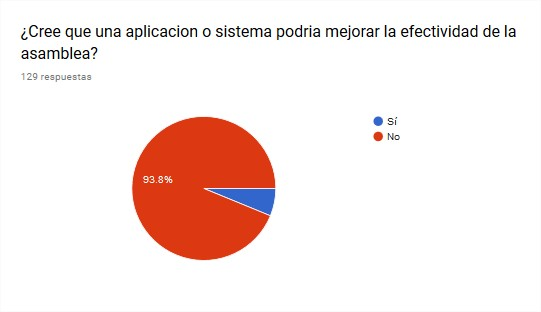
\includegraphics[width=0.7\linewidth]{desarrollo/resultados/imgs/pregunta-1}
	\caption{Gráfica pregunta 1}{\scriptsize \textbf{Fuente:} Imagen propia}
\end{figure}

%%grafo

\begin{figure}[th!]
	\centering
	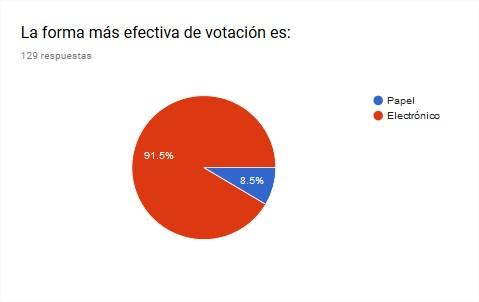
\includegraphics[width=0.7\linewidth]{desarrollo/resultados/imgs/pregunta-2}
	\caption{Gráfica pregunta 2}{\scriptsize \textbf{Fuente:} Imagen propia}
\end{figure}

%%grafo

\begin{figure}[th!]
	\centering
	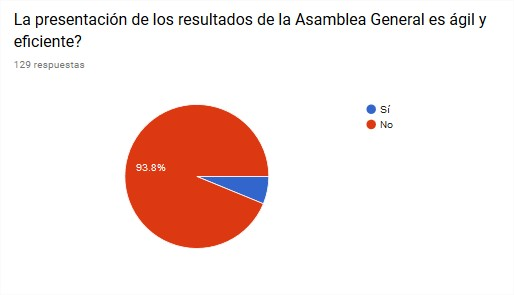
\includegraphics[width=0.7\linewidth]{desarrollo/resultados/imgs/pregunta-3}
	\caption{Gráfica pregunta 3}{\scriptsize \textbf{Fuente:} Imagen propia}
\end{figure}

%%grafo

\begin{figure}[th!]
	\centering
	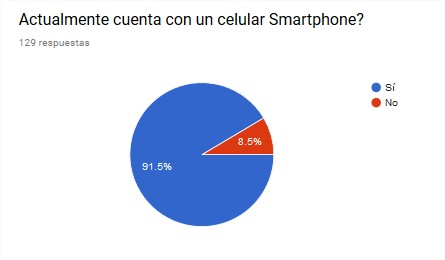
\includegraphics[width=0.7\linewidth]{desarrollo/resultados/imgs/pregunta-4}
	\caption{Gráfica pregunta 4}{\scriptsize \textbf{Fuente:} Imagen propia}
\end{figure}

%%grafo

\begin{figure}[th!]
	\centering
	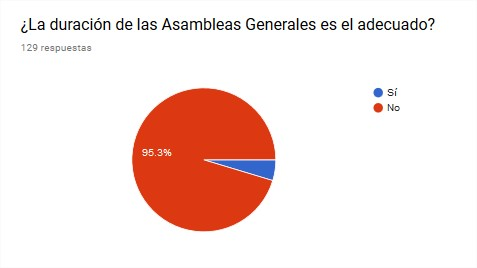
\includegraphics[width=0.7\linewidth]{desarrollo/resultados/imgs/pregunta-5}
	\caption{Gráfica pregunta 5}{\scriptsize \textbf{Fuente:} Imagen propia}
\end{figure}

%%grafo

\begin{figure}[th!]
	\centering
	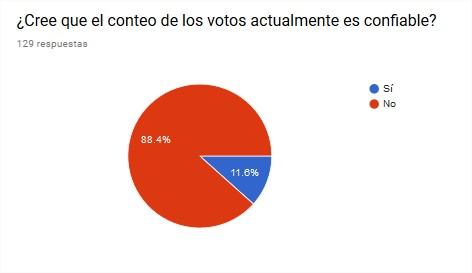
\includegraphics[width=0.7\linewidth]{desarrollo/resultados/imgs/pregunta-6}
	\caption{Gráfica pregunta 6}{\scriptsize \textbf{Fuente:} Imagen propia}
\end{figure}

%%grafo

\begin{figure}[th!]
	\centering
	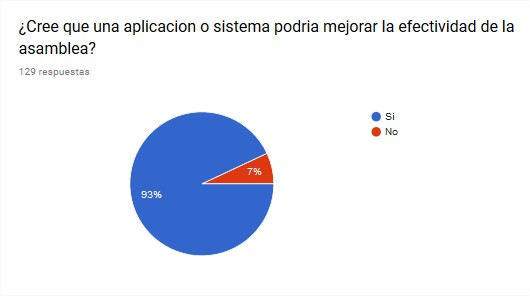
\includegraphics[width=0.7\linewidth]{desarrollo/resultados/imgs/pregunta-7}
	\caption{Gráfica pregunta 7}{\scriptsize \textbf{Fuente:} Imagen propia}
\end{figure}

